% Gráfico de barras — Lote III RAG (Recall@5 com IC 95% Wilson + MRR)
% Requer pgfplots (já no preâmbulo). Rótulos de valor girados 90 graus.
\begin{figure}[htbp]
    \centering
    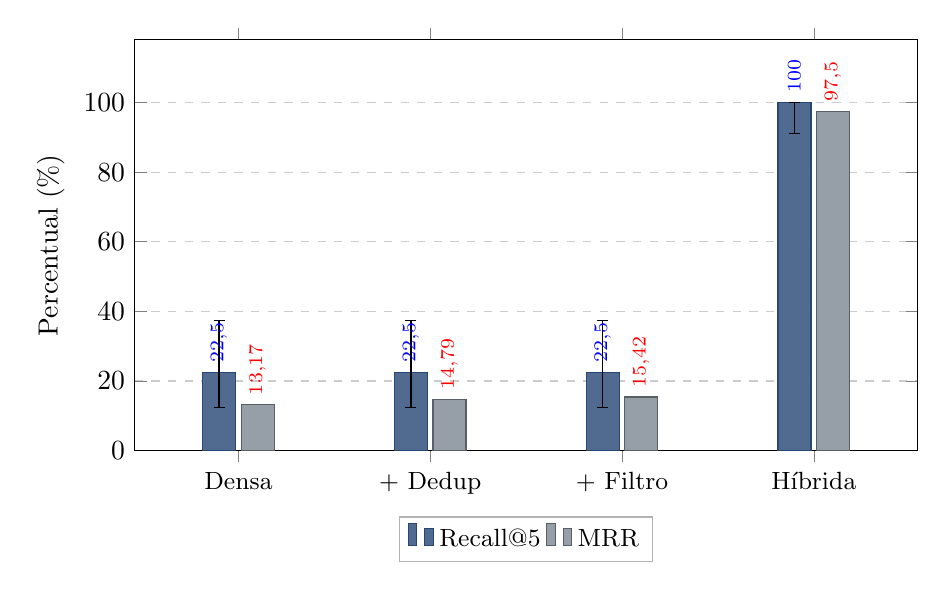
\begin{tikzpicture}
    \definecolor{simRec}{RGB}{38,70,116}
    \definecolor{simMRR}{RGB}{150,158,168}
    \begin{axis}[
        width=0.95\textwidth, height=6.8cm,
        ybar=2pt, bar width=0.42cm,
        ymin=0, ymax=118,
        ytick={0,20,40,60,80,100},
        ylabel={Percentual (\%)},
        xtick={1,2,3,4},
        xticklabels={Densa, {+ Dedup}, {+ Filtro}, Híbrida},
        xticklabel style={font=\small},
        enlarge x limits=0.18,
        ymajorgrids=true, grid style={dashed, black!20},
        legend style={at={(0.5,-0.16)}, anchor=north, legend columns=2,
                      draw=black!30, font=\small},
        nodes near coords,
        every node near coord/.append style={rotate=90, anchor=west, font=\scriptsize,
            /pgf/number format/.cd, use comma, fixed, precision=2},
        clip=false,
    ]
        % --- Recall@5 com IC 95% Wilson (assimétrico) ---
        \addplot+[draw=simRec, fill=simRec!80,
            error bars/.cd, y dir=both, y explicit,
            error bar style={black, line width=0.5pt}]
          table[x=x, y=y, y error plus=ep, y error minus=em] {
            x   y        ep     em
            1   22.50    15.0   10.2
            2   22.50    15.0   10.2
            3   22.50    15.0   10.2
            4   100.00   0.0    8.8
          };
        \addlegendentry{Recall@5}
        % --- MRR (sem IC) ---
        \addplot+[draw=simMRR!60!black, fill=simMRR]
          table[x=x, y=y] {
            x   y
            1   13.17
            2   14.79
            3   15.42
            4   97.50
          };
        \addlegendentry{MRR}
    \end{axis}
    \end{tikzpicture}
    \caption{Lote III --- Recall@5 e MRR por estratégia de recuperação ($n=40$, $k=5$; estratégias cumulativas sobre busca densa). Barras de erro no Recall@5: IC 95\% (Wilson); na configuração híbrida, 91,2--100\%. As três primeiras estratégias mantêm Recall@5 constante (22,5\%) enquanto o MRR melhora com deduplicação e filtro; a busca híbrida por número de ato eleva ambos os indicadores.}
    \label{fig:grafico_rag}
\end{figure}
